\section{Discussions on Error/Bias}

The focus of this study is to analyze how students might go about performing experiments in the department of personal informatics. Although the assignment specified various factors that users needed to take into account, it was vastly general and left the responsibility of design, decision, and analysis completely up to the user. This led to a wide range of different experiments and designs but often times users ran into similar problems.

%\begin{figure}[!t]\centering
%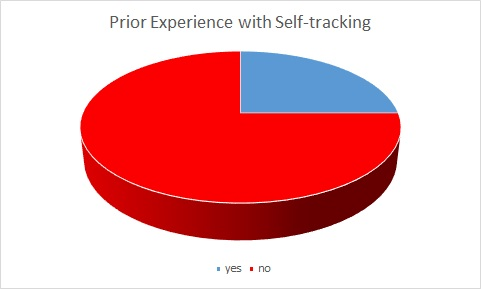
\includegraphics[width=1.0\columnwidth]{images/prior_experience.jpg}
%\caption{\footnotesize Prior experience of participants with self tracking \label{fig:experience} 
%}
%\end{figure}

In general, some participants had difficulty choosing the right design for their experiment. This includes those participants who would have benefited from using randomization rather than a variation of the AB design. Another error that various participants faced was a lack of statistical background and understanding which may have led to some naive conclusions in their report. Finally, an overall poor choice of variables to test was observed in many participants. When choosing a dependent variable, it should be something that is out of the user\textquotesingle s control, and therefore for students who chose sleep or productivity as their dependent variable, for example, because these variables are somewhat under their control (such as setting an alarm clock to wake up) these variables are not entirely dependent.  

Another concern for the majority of the participants of these studies were confounding factors that heavily affected their data. For example, the last week of the experiment happened to fall during spring break. As mentioned previously, most participants dealt with variables such as productivity and sleep, which for most is highly diminished and increased respectively during break. Other factors include participants who travelled or were sick during the experiment. These factors seemed to greatly impact the data for most participants.

Finally, most participants felt the study was too short and wished they could do it for longer, stating that 28 days was too little time to garner enough data points to have any statistically significance towards their hypothesis. Participants stated that due to the short time span, events such as exams, presentations, etc had bigger effects on their data than they would in the long run. 
